\checkoddpage
\ifoddpage\cleartoevenpage\fi
\thispagestyle{empty}
\vspace*{\fill}
    \begin{center}
    \resizebox{0.25\columnwidth}{!}{\includestandalone{figures/confucius}}
    \end{center}
\vspace*{\fill}
%The Master said, 'Look at the means a man employs, observe the path he takes and examine where he feels at home. In what way is a man's true character hidden from view? In what way is a man's true character hidden from view?' -- Confucius (The analects of Confucius book II, verse 9)
\chapter[Phase Space and Experimental Comparisons][Phase Space and Experiments]{Phase Space and Experimental Comparisons}\label{ch:tlsphase}
\lofchap{Phase Space and Experimental Comparisons}
\chapterprecis{Identifying possible TLS candidates by comparing model results to experimental coupling variables such as the ground to first excited state energy splitting and dipole moment.}

\thought{To understand the properties of} a delocalised oxygen, we have considered confining aluminium atoms in both a line and in a plane.
In reality, aluminium atoms will surround the oxygen in all three dimensions.

This chapter expands on the \lin{2D} model discussed in \cref{sec:2d}, adding an additional aluminium pair in \cref{sec:tls}, which extends oxygen confinement into three dimensions (with six aluminum atoms), whilst still projecting oxygen delocalisation on a plane.
Although in general an oxygen can delocalise in three dimensions, for this investigation we focus on an effective \lin{2+1D} model, minimising both computational and descriptive complexity while still modelling the relevant behaviour of the system.
\Cref{ch:threedee} will consider possible ambiguities to this approach when juxtaposing it with a \lin{3D} implementation.
The following sections then apply the \lin{2+1D} model and compare delocalised oxygen responses to experimental TLS data.
\Cref{sec:smax} discusses qubit--TLS coupling and \cref{sec:strain} observes the effect of mechanical strain.

\section{TLS Defect Confined in Three Dimensions}\label{sec:tls}

Two more confining atoms are now added into the system in the $z$ direction labelled as $\abs{Z}$.
Interactions with these atoms in the third dimension are now considered, although the model is still two dimensional (\ie \lin{2+1D}); thus oxygen continues to be confined to the $xy$ plane.
An illustration of this cluster configuration is displayed in \cref{fig:cage} and representations of the cage potential and oxygen wavefunctions are shown in \cref{fig:wfstackA} for A and \cref{fig:wfstackB} for B type defects.

\begin{figure}[htp]
  \resizebox{0.6\textwidth}{!}{\includestandalone{figures/cage}}
  \caption[\lin{2+1D} Cluster Illustration]{\label{fig:cage}Illustration of an idealised cluster producing a void in \lin{3D}. Six cage aluminium atoms \resizebox{0.5em}{!}{\includegraphics{figures/aluminium}} sit in pairs on each cardinal axis, equidistant from the origin. Separation distances $\abs{X}$ and $\abs{Y}$ are labeled for reference (see text). The plane \begin{tikzpicture}[baseline=-0.7ex]\filldraw [Set1-5-1,fill=Set1-5-1!80,fill opacity=0.7] (0,-0.1) -- (0.5,-0.1) -- (0.5,0.1) -- (0,0.1) --cycle;\end{tikzpicture} at $z=0$ is a representation of the \lin{2D} delocalisation of an oxygen atom.}
\end{figure}

\begin{figure}[p]
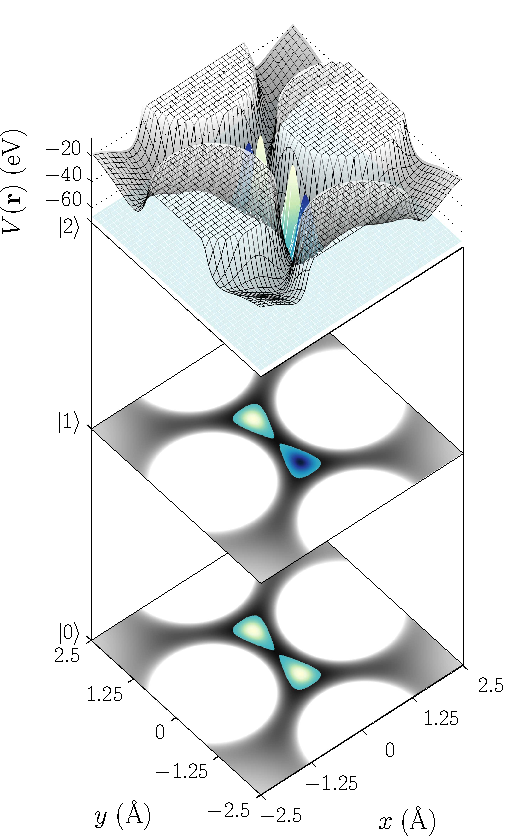
\includegraphics[width=0.85\textwidth]{figures/wfstackA}
\caption[A Type Energy States]{\label{fig:wfstackA}Cage potential and the lowest three eigenfunctions of a cluster with the values $\abs{X}=1.53, \: \abs{Y} = 2.52, \: \abs{Z} = 2.25$ \AA. The top image in the stack is presented with the apparent `depth' of the potential well on the $z$-axis and the second excited state $\ket{2}$ scaled accordingly. Ground $\ket{0}$ and first excited $\ket{1}$ states are displayed in a projected representation underneath. This cluster configuration is representative of an A type defect (see \cref{fig:Atype}); with a ground to first excited state splitting of $E_{01} = 8.1$ GHz and a ground to second excited state splitting of $E_{02} = 202.2$ THz.}
\end{figure}

\begin{figure}[p]
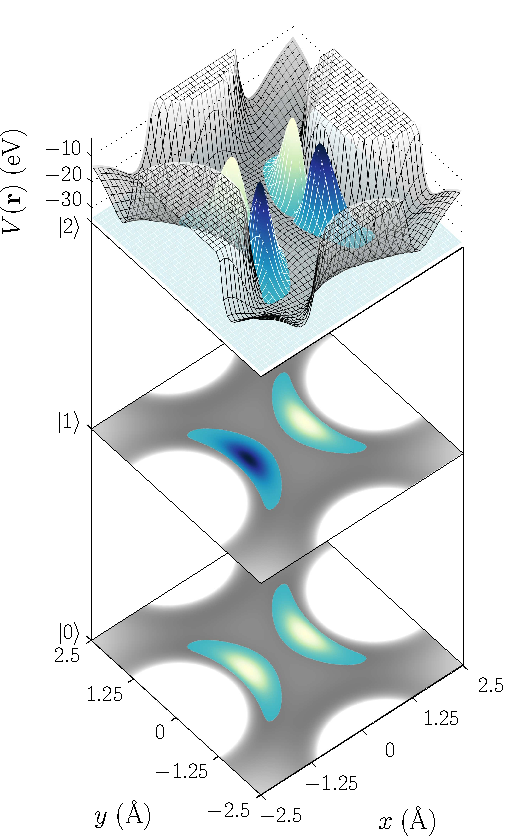
\includegraphics[width=0.85\textwidth]{figures/wfstackB}
\caption[B Type Energy States]{\label{fig:wfstackB}Cage potential and the lowest three eigenfunctions of a cluster with the values $\abs{X}=2.38, \: \abs{Y} = 3.19, \: \abs{Z} = 2.75$ \AA. The top image in the stack is presented with the apparent `depth' of the potential well on the $z$-axis and the second excited state $\ket{2}$ scaled accordingly. Ground $\ket{0}$ and first excited $\ket{1}$ states are displayed in a projected representation underneath. This cluster configuration is representative of a B type defect (see Figure \ref{fig:Btype}); with a ground to first excited state splitting of $E_{01} = 8.4$ GHz and a ground to second excited state splitting of $E_{02} = 36.3$ THz.}
\end{figure}

The selection of a fixed $\abs{Z}$ distance changes the phase landscape in a manner that can be qualitatively extrapolated between two arbitrary values even a few angstroms apart.
Values of $\abs{Z} = 2.75$ \AA\ (\cref{fig:xi275}) and $\abs{Z} = 2.25$ \AA\ (\cref{fig:xi225}) have been chosen to analyse in detail.

TLS behaviour can be observed on both maps and each value of $\abs{Z}$ has been selected based on model parameters.
Oxygen confinement occurs for $\abs{Z}$ values lower than $2.25$ \AA\ (\ie $E_{01} \gg 100$ GHz).
$\abs{Z}$ values larger than $2.75$ \AA\ show similar phase behaviour to that of \cref{fig:xiunbound}, which in completely unbound in $z$.
Large $\abs{Z}$ separation distances also decrease the validity of the \lin{2+1D} model, in addition: the radial distribution analysis in \cref{sec:gr} suggests large separation distances for nearest neighbour atoms have a low probability of occurrence.

\begin{figure}[htp]
  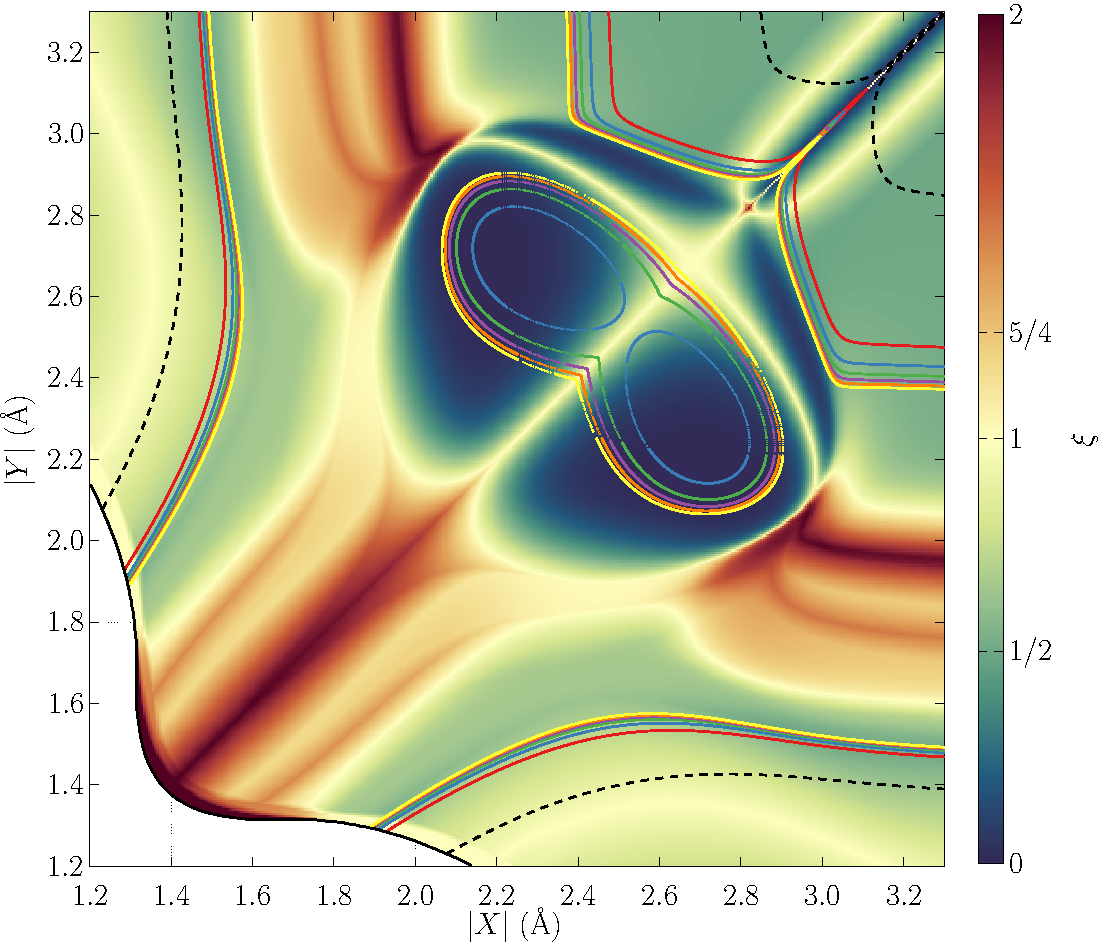
\includegraphics[width=\textwidth]{figures/xi275}
  \caption[$\xi$ Metric Phase Map, With $\abs{Z} = 2.75$ \AA]{\label{fig:xi275}Map of the $\xi$ metric of the delocalized oxygen model confined in two dimensions. The $\abs{X}$ and $\abs{Y}$ axes represent aluminium pair positions with $\abs{Z} = 2.75$ \AA. \plotline{line width=1.5pt,dashed} represents a minimum resolvable energy splitting of $10$ kHz. The white (blank) section indicates where the aluminium atoms are so close, the oxygen confinement region no longer exists. Overlayed contour lines corresponding to $E_{01} = 0.5\!-\!10$ GHz (red to yellow) are comparable to existing experimental qubit results. Cases where quad-degeneracy exists are denoted as dotted rather than solid contours.}
\end{figure}

\begin{figure}[htp]
  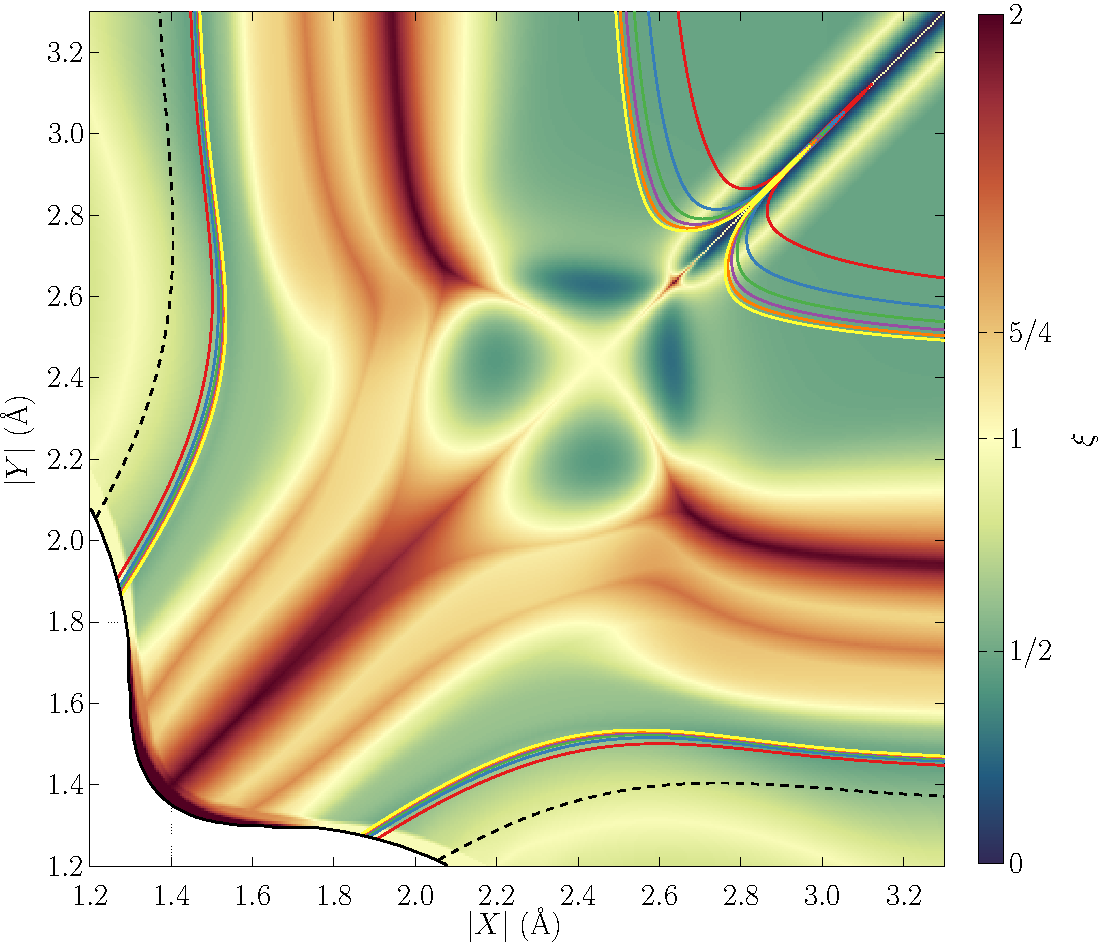
\includegraphics[width=\textwidth]{figures/xi225}
  \caption[$\xi$ Metric Phase Map, With $\abs{Z} = 2.25$ \AA]{\label{fig:xi225}Map of the $\xi$ metric of the delocalized oxygen model confined in two dimensions. The $\abs{X}$ and $\abs{Y}$ axes represent aluminium pair positions with $\abs{Z} = 2.25$ \AA. \plotline{line width=1.5pt,dashed} represents a minimum resolvable energy splitting of $10$ kHz. The white (blank) section indicates where the aluminium atoms are so close, the oxygen confinement region no longer exists. Overlayed contour lines corresponding to $E_{01} = 0.5\!-\!10$ GHz (red to yellow) are comparable to existing experimental qubit results.}
\end{figure}

As the pair separation distance $\abs{Z}$ decreases, the tetra-well ($\xi=0$) regimes diminish in size and no longer exhibit TLS behaviour.
This suggests that quad-degenerate defects, whilst quite rare in phase space already, are extremely rare in reality.
For one to exist in a junction, the amorphous layer would have to be disordered in such a way that an oxygen atom's nearest neighbour atom pair exists at a distance greater that $\sim 3$ \AA\ along one orthogonal basis vector.

Whilst this configuration of six cage aluminium atoms on cardinal axes around a central oxygen is still an idealised system, \cref{fig:xi225} is confined in all three spatial dimensions with pragmatic distances and is therefore considered to be the most `realistic' representation of the TLS phase space for the \lin{2+1D} model.
TLS candidates lie well within hemi-tetra- ($\xi=1/2$) domains, are not mired by higher energy level complexities (\ie quad-degeneracies) and can be identified as A type and B type defects separated by an (an)harmonic boundary.

Phase space is also dominated on this map with $\xi=5/4$ (harmonic) and $\xi=2$ (unique ground state) domains where the oxygen atom can be considered under the spatial harmonic approximation (\ie localised).
This is significant, as TLS observations in experiments are not statistically dense.
We expect few defects in the junction compared to the number of atoms extant.

\section{Charge Dipoles}\label{sec:dipole}

As stated in \cref{sec:phenom}, another important experimentally measurable property of the TLS is its strong electric dipole moment.
Using the same $\abs{X}, \: \abs{Y}$ and $\abs{Z}$ parameters from the phase maps in the previous section, the dipole elements in the $x$ direction $\wp_x$, and the $y$ direction $\wp_y$ can be calculated via \cref{eq:dipole}.
\Cref{fig:dipole275} shows the same phase space as \cref{fig:xi275}, where $\abs{Z} = 2.75$ \AA, and \cref{fig:dipole225} matches \cref{fig:xi225}, where $\abs{Z} = 2.25$ \AA.
The colourmap for both figures now represent dipole strengths of each cluster configuration rather than energy level splittings (represented through the $\xi$ metric).
These computed dipole moments correspond well to observed values, assuming $\mathcal{O}$(nm) junction widths~\cite{Martinis2005, Cole2010}.

\begin{figure}[htp]
  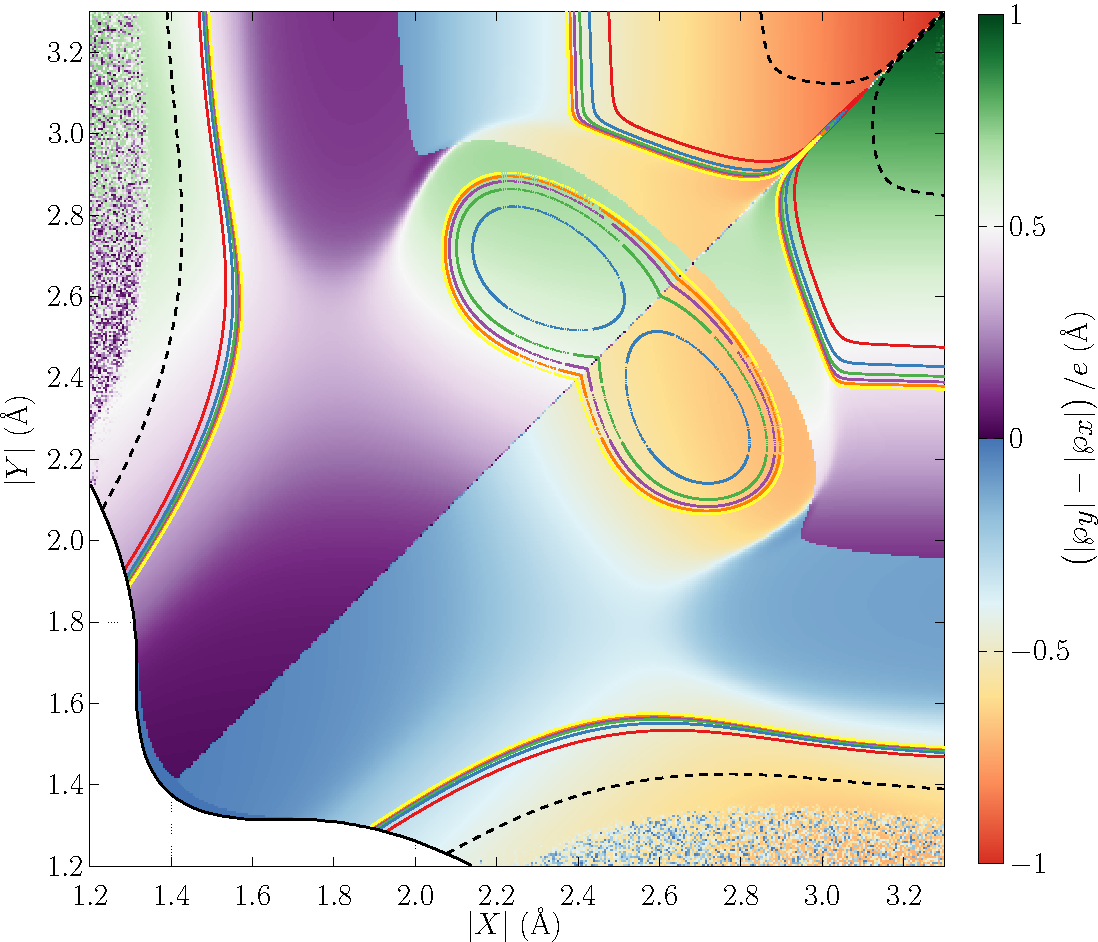
\includegraphics[width=\textwidth]{figures/dipole275}
  \caption[Dipole Phase Map, With $\abs{Z} = 2.75$ \AA]{\label{fig:dipole275}The difference between the absolute dipole moment (in $x$- and $y$-directions) over the same range for $\abs{Z} = 2.75$ \AA. We see either $\abs{\wp_x}$ (red) or $\abs{\wp_y}$ (green) dominated behaviour in the tetra- and hemi-tetra- domains but none in other regions.}
\end{figure}

\begin{figure}[htp]
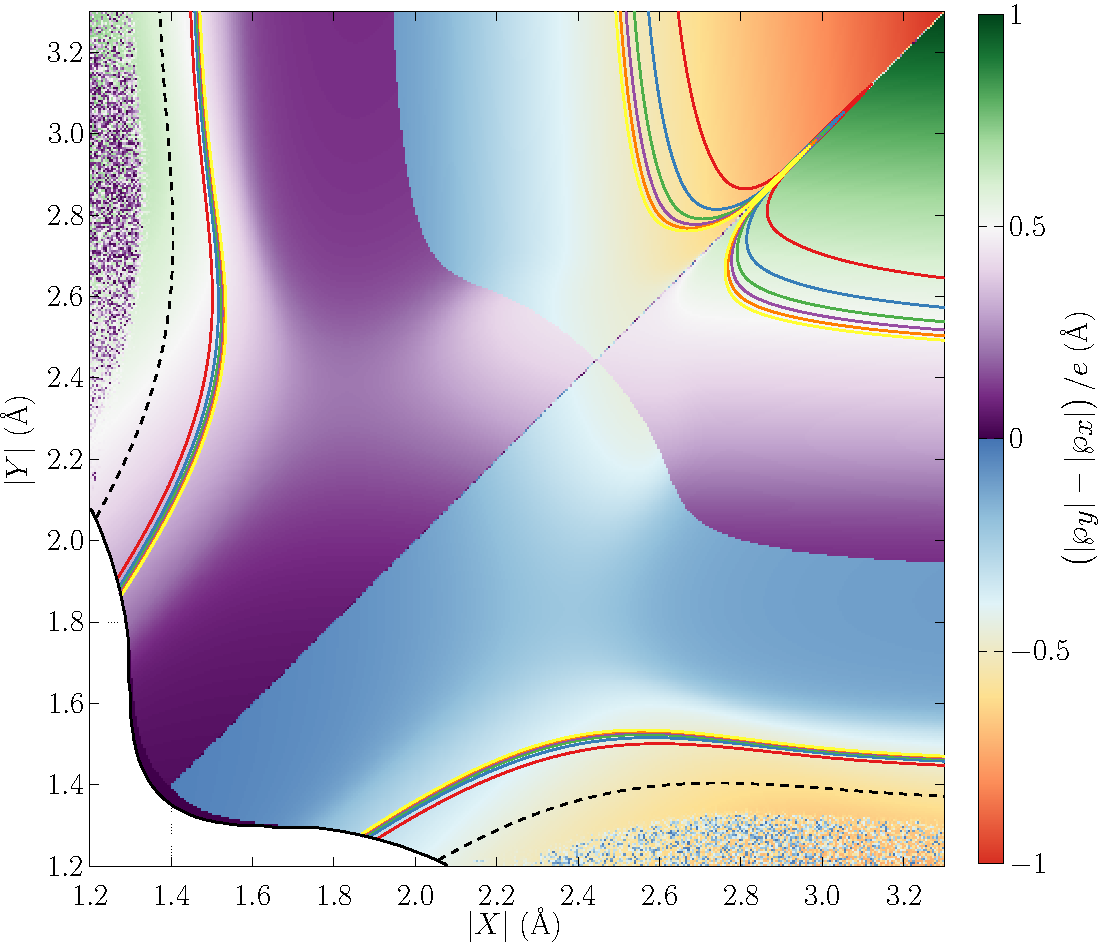
\includegraphics[width=\textwidth]{figures/dipole225}
  \caption[Dipole Phase Map, With $\abs{Z} = 2.25$ \AA]{\label{fig:dipole225}The difference between the absolute dipole moment (in $x$- and $y$-directions) over the same range for $\abs{Z} = 2.25$ \AA. We see either $\abs{\wp_x}$ (red) or $\abs{\wp_y}$ (green) dominated behaviour in the tetra- and hemi-tetra- domains but none in other regions.}
\end{figure}

The dipole moments are presented as $\left(\abs{\wp_y}-\abs{\wp_x}\right)/e$ rather than separate plots because the dipole elements are discontinuous at the bifurcation points (\ie when $\abs{\wp_x}>0, \abs{\wp_y}=0$ and \textit{vice versa}).
Comparing these plots to the phase maps in \cref{sec:tls}, it is apparent that only the tetra- and hemi-tetra- domains ($\xi < 1$) exhibit a dipole response---which is appropriate for our model as $E_{01}$ splittings representative of a TLS only appear in these regions.
Localised oxygen atoms ($\xi > 1$) are also expected to not elicit dipole behaviour.
With this information, the domain boundaries and bifurcations on each phase map can now be fully explained.

Two variables alter the landscape: dipole and potential.
Clusters with tight $z$ confinement (those without tetra-well regions such as $\abs{Z} = 2.25$ \AA) have four unique regions where a TLS may reside.
The dipole direction dominates two of these domains: an A type region when the confining pair is collinear to the dipole, and a B type region when the confining pair is perpendicular.
A symmetry bifurcation (at $\abs{X} = \abs{Y}$) separates the dipole domains into four regions which can therefore be identified in terms of dipole moment ($\abs{\wp_x}$ or $\abs{\wp_y}$) and defect type (A or B).

Clusters without as much $z$ confinement (such as $\abs{Z} = 2.75$ \AA) exhibit tetra-well behaviour: generating two additional regions.
Tetra-well domains, as discussed in \cref{sec:phaseanalysis}, are caused when the confining pair of aluminium atoms start interacting with the defect pair (and hence the oxygen as well).
If we consider the A type, $\abs{\wp_y}$ domain in \cref{fig:dipole275}, it is clear that the dominant dipole direction remains constant as $\abs{X}$ separation is in increased and the tetra-well domain is entered.
The same $\abs{X},\abs{Y}$ parameters on \cref{fig:dipole225} cross a bifurcation line, changing dipole direction and the model indicates B type defect properties.
Increased confinement in $z$ induces a deeper potential well in the $xy$ plane and removes any major landscape changing contributions from the confining atom pair---\textit{effectively reducing the model back to a \lin{1D} description}.
A cluster with a comparatively shallow potential that generates tetra-well domains does so when conditions are advantageous for an A type confinement pair to become a B type defect pair (a dipole direction change is not required for this to occur).
A trace like the $\abs{Y} = 2.5$ \AA\ (labelled A) on \cref{fig:xiunbound} (and an associated eigenspectrum response similar to \cref{fig:tetraspectrum}) is an example of this behaviour.
If we do not consider the small portion of quad-degenerate defects in this domain; the measurable properties (\ie $E_{01}$ and dipole strength) tetra-well, B type, $\abs{\wp_y}$ TLSs are identical to B type, $\abs{\wp_y}$ TLSs that reside in a hemi-tetra-well domain.


\section{Qubit Coupling}\label{sec:smax}

To compare our TLS model directly to experiments, we have assumed that our JJ lies within a phase qubit, although the model applies equally for any device comprised of amorphous junctions.
The measurable signal of a TLS in a phase qubit is the resonance of the TLS and qubit splitting energy, $E_{01}$, with the qubit-TLS coupling.
For the phase qubit~\cite{Martinis2005}, the qubit-TLS coupling $S_{max}$ \cref{eq:smax} is a function of $E_{01}$ and $\wp$~\cite{Kofman2007}, the effective dipole moment due to an electric field applied in the direction of delocalization.
Throughout this discussion we assume a junction width $w = 2$ nm and capacitance $C = 850$ fF.

The dipole magnitudes in \cref{fig:dipole275,fig:dipole225} are calculated against the electron charge for simplicity, although as we are discussing an oxygen atom, the effective charge on the atom may in fact be larger.
Using our Josephson junction DFT models from \cref{ch:junctions}, we partition the charge density associated with atoms across the lattice into Bader volumes~\cite{Tang2009}.
The charge enclosed within each Bader volume is an adequate approximation to the total electronic charge of an atom.
An average value of $1.395\pm0.006 \; e$ is found for oxygen atoms in a junction comprised of \ce{AlO_{1.25}} at a density of 0.8 times that of corundum. We can use this value such that
\begin{equation}
\widetilde{\wp_x} = 1.4e\wp_x
\end{equation}
(for a dipole in the $x$ direction) to gain a better estimate of $S_{max}$.

In \cref{fig:smax225} we plot contour lines representing constant values of $E_{01}$ corresponding to the purview of qubit resonant frequencies observed experimentally  for constant values of $\abs{Z} = 2.25$ \AA.
The $S_{max}$ \cref{eq:smax} response to these frequencies is plotted as a function of $\abs{X}$, in which we see maximum coupling strengths which correspond exceptionally well with experimental observations~\cite{Lupascu2009, Shalibo2010, Cole2010}.
The most comprehensive of these studies (\onlinecite{Shalibo2010}) measures $S_{max}$ values of $3$--$45$ MHz.

\begin{figure}[htp]
\resizebox{0.9\textwidth}{!}{\includestandalone{figures/smax225}}
\caption[$S_{max}$ Couplings]{\label{fig:smax225}Coupling strength to a fictitious phase-qubit $S_{max}$ as a function of $\abs{X}$ in the domains where both dipoles $\abs{\widetilde{\wp}_{x,y}}$ are dominant (see \labelcref{eq:smax}) for a set of constant $E_{01}$ splitting frequencies and $\abs{Z} = 2.25$ \AA.}
\end{figure}

Whilst the $S_{max}$ response is neither smooth nor singular over the investigated phase space, the value range is notably small.
\Cref{fig:smaxz} shows the range of $S_{max}$ couplings for all $E_{01}=8$ GHz configurations calculated with confinements in $\abs{Z}$ from $2.25$ \AA\ to unbound and $\abs{X}$ (hence $\abs{Y}$ as well from symmetry arguments) from $1.2$ to $4$ \AA.
The entire range of $S_{max}$ values is only $60$ MHz wide, which suggests an explanation as to why large couplings (of order $500$ MHz for example) have not been seen experimentally.

\begin{figure}[htp]
\resizebox{\textwidth}{!}{\includestandalone{figures/smaxz}}
\caption[$S_{max}$ Response Range]{\label{fig:smaxz}$S_{max}$ response range for a constant $E_{01}$ splitting frequency of $8$ GHz as a function of $\abs{Z}$ separation. Each box on the figure represents the minimum to maximum $S_{max}$ values in both $\abs{\wp_{x}}$ and $\abs{\wp_{y}}$ dominant domains over the phase space of $\abs{X}$ distance separations. The box at $\abs{Z} = 2.25$ \AA\ represents all $E_{01} = 8$ GHz values on \cref{fig:smax225} for example. Median values are plotted as solid lines inside each box. Orange boxes represent degenerate regions and blue boxes indicate quad-degenerate regions.}
\end{figure}

\section{Strain Response}\label{sec:strain}

Unusually long coherence times of strongly coupled defects are a key observation of TLS-qubit experiments~\cite{Neeley2008, Lisenfeld2010a}.
As our model assumes a charge-neutral defect\footnote{More specifically: the defect is globally charge neutral, whilst the oxygen possess a net charge.}, coherence times are linked to the dipole element (for charge noise) and the strain response (for phonons).
Mechanical deformation of a phase-qubit has recently been observed directly~\cite{Grabovskij2012}, which we can mimic in our \lin{2+1D} model by introducing a series of deformations onto the cluster, and subsequently measure the $E_{01}$ response.

Deformation types that were tested are depicted in \cref{fig:strainxa}.
All deformations were tested in each of the four hemi-tera- regions discussed in \cref{sec:tls}, not only in the $x$-direction as shown, but also in $y$.
Of the tested deformations we find the response of one (translation of $\abs{X}$, highlighted in \cref{fig:strainxa}) to be $10^5$ times stronger than the others.
Such a deformation corresponds to a translation of both aluminium atoms in the same direction and relative to the oxygen, along the axis of the dominant dipole.
This suggests an explanation for the long TLS coherence times, as a delocalized oxygen is only sensitive to a small subset of available phonon modes (as well as coupling to charge noise only through its electric dipole).

\begin{figure}[htp]
  \resizebox{\textwidth}{!}{\includestandalone{figures/strainx}}
  \caption[Model Strain Response]{\label{fig:strainx}\label[figurea]{fig:strainxa}\label[figureb]{fig:strainxb}\label[figurec]{fig:strainxc} (a) Depiction of a number of deformations which were applied to the aluminium atoms in the $x$-$y$ plane. The response of one of the strain types is orders of magnitude larger than the others (highlighted), which is indicative of an optical phonon mode, generating extremely large frequency splittings for picometer deformations. A deformation range of $10$ fm was applied at points along 8 GHz contours (corresponding to phase qubit-TLS coupling strengths), with $\abs{Z}=2.5$ \AA, yielding responses that are both hyperbolic and symmetric. (b) Over the range $2\!-\!10$ fm the response is linear with a strain gradient, shown in (c) for both the A and B type defects in $\abs{\wp_x}$ domains.}
\end{figure}

\Cref{fig:strainxb} shows this response for the optical mode (at positions corresponding to phase qubit-TLS coupling strengths $\sim 8$  GHz where $\abs{Z}=2.5$ \AA), displaying a characteristic hyperbolic response which is typical of a two-level system.
This compares well with the observed strain response in \onlinecite{Grabovskij2012}.
Fitting the data in the inset of \cref{fig:strainxb} using the harmonic approximation (assuming an optical mode), we obtain characteristic frequencies in the range $0.3\!-\!1.0$ THz.
This is well above the energy of typical qubit experiments, again limiting the coupling of the defect to phonons; although it is still possible that slow noise fluctuations couple to the defect via a similar deformation (\textit{vide infra}).
Finally, \cref{fig:strainxc} shows the linear strain gradient plotted along the $E_{01}/h = 8$ GHz contour for the tetra- and hemi-tetra- regions in the $\abs{\wp_x} \neq0, \abs{\wp_y}=0$ domains (when $\abs{Z} = 2.5$ \AA)---which may be an important property for a future model describing TLS-phonon coupling.

Whilst the large, hyperbolic response of the $\abs{X}$ translation seems to be observed in experiments, it is not the only strain mode possible.
Most deformation types in \cref{fig:strainxa} do not exhibit any substantial change to defect properties, although two types (depicted again in \cref{fig:straina}) show an active response over a length change $\Delta L$ of $1$ pm.
Four clusters are chosen that lie on the $8$ GHz contour when $\abs{Z} = 2.25$ \AA, indicated as (b), (c), (d) and (e) in \cref{fig:straina}.
As can be seen in \cref{fig:dipole225}, each of these cases are within a $\abs{\wp_x}$ dominant domain.

\begin{figure}[p]
\resizebox{0.75\textwidth}{!}{\includestandalone{figures/strain}}
\caption[Strain Response of TLS Clusters]{\label{fig:strain}\label[figurea]{fig:straina}Strain response of four candidate TLS clusters. (a) Left: depictions of two deformation types that show active responses. A dilation: where an $\abs{Y}$ (shown) or $\abs{X}$ pair is stretched from their original position and a translation: where an $\abs{Y}$ (shown) or $\abs{X}$ pair is moved from their original position. Right: locations along the $8$ GHz contour from the $\abs{Z} = 2.25$ \AA\ phase maps. Each case is deformed and translated in both $x$ and $y$ directions by $\pm 1$ pm and plotted as (b), (c), (d) and (e). Dilation of $\abs{X}$ \plotline{line width=2pt,color=Set1-5-1}, Translation of $\abs{Y}$ \plotline{line width=2pt,dashed,color=Set1-5-2}, Dilation of $\abs{Y}$ \plotline{line width=2pt,dotted,color=Set1-5-3}. Note that all four cases lie in the $\abs{\wp_x}$ dominant domain (see \cref{fig:dipole225}). Translation of $\abs{X}$ is not shown on any graph as its' $E_{01}$ response is of $\sim\!10^4$ GHz over ($\Delta L$) for all cases.  }
\end{figure}

Clusters (b) and (c) are both identified as A type defects and are insensitive to $\abs{X}$ dilation and $\abs{Y}$ translation.
Dilation of $\abs{Y}$ for these defects is a different way of saying `extending the defect pair separation'---which has been described in the above sections.
The intensity of the response however is noticeably larger as the confinement distance ($\abs{X}$) is increased.

B type defects, labelled (d) and (e), respond discordantly depending on their configuration.
Dilation in $\abs{Y}$, whilst a sizable strain source for A type configurations, initiates no response from the (e) configuration at all.
B type defects located at this position in phase space have their defect pair in $\abs{X}$, and point (e) specifically is confined with $\abs{Y} = 3.1$ \AA.
As discussed in the sections above, this separation distance is close to being practically unbound.
Point (d) on the other hand has a tighter separation distance and begins to confine the system.
Dilation in $\abs{X}$ responds in the opposite manner effectively: expanding defect separation distance whilst keeping the confinement distance static ultimately confines the wavefunction.
The final response that the B type defects respond to is $\abs{Y}$ translation.
As point (e) is essentially unbound in $\abs{Y}$ we do not expect any response from a strain of this magnitude.
Point (d) on the other hand is interacting with its tighter confinement distance, with the TLS dipole collinear to the $\abs{X}$ direction.
Translation of $\abs{Y}$ forces local minima of the potential landscape from points on the $x$ axis to locations off axis, yet still within the minima rings about the aluminium atoms.
In other words, the wavefunction is slightly rotated around the defect axis.

\section{Summary of the Low Dimensional TLS Model}\label{sec:lowsummary}

Despite the extreme idealisation of this model, it allows the prediction of experimentally measured properties of strongly coupled TLSs with atomic positions as the only input parameters and therefore shows as a proof of concept that these defects can arise in \ce{AlO_x} without any alien species present.

Even when considering delocalisation in only two dimensions, a range of different behaviour can be seen.
The existence of effective two-state systems can come about through different potential shapes, which in turn arise due to various atomic position configurations.
To understand these different configurations, we consider both the symmetries of the eigenspectrum and the effective charge dipole of the defect.

We find that two-level systems with equivalent properties to those seen in experiments can be formed from atomic configurations which are entirely consistent with the material properties of amorphous aluminium oxide barriers.
Most interestingly we find that the expected qubit-TLS coupling strength and the TLS strain response correspond very well to that observed experimentally.

A complication that occurs with phenomenological models that attempt to describe TLS behaviour is their free parameter count is high enough to describe all facets of the observed experimental parameters without being distinguishable from other, non-complimentary models~\cite{Cole2010}.
Whilst this delocalised oxygen model only uses one type of parameter as input (atomic positions), it still requires an $x, y, z$  coordinate set for up to $6$ cage atoms.
Realistic values for the atomic positions obtained by the junction model in \cref{ch:junctions} are still yet to be applied to the model, which may require more than $6$ atoms and thus even more free parameters.
A method to account for this parameter runaway is discussed later in the next chapter. 